\documentclass[10pt]{article}
% \usepackage{geometry}
% \geometry{margin=0.2in}
\usepackage[utf8]{inputenc}

\nonstopmode
% \usepackage{minted}[cache=false]
\usepackage{graphicx} % Required for including pictures
\usepackage[figurename=Figure]{caption}
% \usepackage{float}    % For tables and other floats
\usepackage{amsmath}  % For math
\usepackage{amssymb}  % For more math
\usepackage{fullpage} % Set margins and place page numbers at bottom center
% \usepackage{paralist} % paragraph spacing
% \usepackage{subfig}   % For subfigures
%\usepackage{physics}  % for simplified dv, and 
% \usepackage{enumitem} % useful for itemization
% \usepackage{siunitx}  % standardization of si units
\usepackage{hyperref}
% \usepackage{mmacells}
% \usepackage{listings}
% \usepackage{svg}
% \usepackage{xcolor, soul}
\usepackage{bm}
\usepackage{braket}

% \usepackage{setspace}
% \usepackage{listings}
% \usepackage{listings}
% \usepackage[autoload=true]{jlcode}
% \usepackage{pygmentize}

% \definecolor{cambridgeblue}{rgb}{0.64, 0.76, 0.68}

% \sethlcolor{cambridgeblue}

\usepackage[margin=1.8cm]{geometry}
\newcommand{\C}{\mathbb C}
\newcommand{\D}{\bm D}
\newcommand{\R}{\mathbb R}
\newcommand{\Q}{\mathbb Q}
\newcommand{\Z}{\mathbb Z}
\newcommand{\N}{\mathbb N}
\newcommand{\PP}{\mathbb P}
\newcommand{\A}{\mathbb A}
\newcommand{\F}{\mathbb F}
\newcommand{\1}{\mathbf 1}
\newcommand{\ip}[1]{\left< #1 \right>}
\newcommand{\abs}[1]{\left| #1 \right|}
\newcommand{\norm}[1]{\left\| #1 \right\|}

\def\Tr{{\rm Tr}}
\def\tr{{\rm tr}}
\def\Var{{\rm Var}}
\def\calA{{\mathcal A}}
\def\calB{{\mathcal B}}
\def\calD{{\mathcal D}}
\def\calE{{\mathcal E}}
\def\calG{{\mathcal G}}
\def\from{{:}}
\def\lspan{{\rm span}}
\def\lrank{{\rm rank}}
\def\bd{{\rm bd}}
\def\acc{{\rm acc}}
\def\cl{{\rm cl}}
\def\sint{{\rm int}}
\def\ext{{\rm ext}}
\def\lnullity{{\rm nullity}}
% \DeclareSIUnit\clight{\text{\ensuremath{c}}}
% \DeclareSIUnit\fm{\femto\m}
% \DeclareSIUnit\hplanck{\text{\ensuremath{h}}}


% \lstdefinelanguage{julia}%
%   {morekeywords={abstract,break,case,catch,const,continue,do,else,elseif,%
%       end,export,false,for,function,immutable,import,importall,if,in,%
%       macro,module,otherwise,quote,return,switch,true,try,type,typealias,%
%       using,while},%
%    sensitive=true,%
% %    alsoother={$},%
%    morecomment=[l]\#,%
%    morecomment=[n]{\#=}{=\#},%
%    morestring=[s]{"}{"},%
%    morestring=[m]{'}{'},%
% }[keywords,comments,strings]%

% \lstset{%
%     language         = Julia,
%     basicstyle       = \ttfamily,
%     keywordstyle     = \bfseries\color{blue},
%     stringstyle      = \color{magenta},
%     commentstyle     = \color{ForestGreen},
%     showstringspaces = false,
% }

% $
\begin{document}
\begin{center}
	\hrule
	\vspace{.4cm}
	{\textbf { \large CAS PY 452 --- Quantum Physics II}}
\end{center}
 Emmy Blumenthal \hspace{\fill} \hspace{\fill}  \textbf{} Discussion Notes\  \\
\textbf{Date:}\  October 12, 2022   \hspace{\fill} \textbf{Email:}\ emmyb320@bu.edu

\vspace{.4cm}
\hrule

\section*{Perturbing two harmonic oscillators}


% \paragraph{Problem statement:}

% Consider two identical bosons in uncoupled identical quantum harmonic oscillators; that is, consider the following Hamiltonian:
% \begin{align}
% 	\hat H_0
% 	=
% 	\frac{\hat p_1^2}{2m}
% 	+
% 	\frac{\hat p_2^2}{2m}
% 	+
% 	\frac{1}{2} m \omega^2 \hat x_1^2
% 	+
% 	\frac{1}{2} m \omega^2 \hat x_2^2.
% \end{align}
% Now perturb the Hamiltonian $\hat H = \hat H_0 + \hat H'$ with,
% \begin{align}
% 	\hat H' = \lambda \hat x_1^2,
% \end{align}
% where $\lambda \ll m \omega^2/2$.
% Find the first and second-order corrections to the energy of the first excited state (which is doubly-degenerate), and find the first-order corrections to the first excited state.
% % In discussion, we considered perturbations to the first excited state (which is doubly degenerate).
% % This problem could be solve trivially and exactly, but we're going to get a little practice.

% \paragraph{Solution:}

% We will use ladder operators to compute inner products; if any of this is unclear, you should look at the discussion notes from Oct. 5.
% Here are some identities for reference:
% \begin{align}
% 	\hat a
% 	=
% 	\sqrt{\frac{m \omega}{2 \hbar}} ( \hat x + \frac{i}{m\omega}\hat p),
% 	\qquad
% 	\hat a^\dagger
% 	=
% 	\sqrt{\frac{m \omega}{2 \hbar}} ( \hat x - \frac{i}{m\omega}\hat p),
% \end{align}
% \begin{align}
% 	\hat x = \sqrt{
% 		\frac{\hbar}{2m \omega}
% 	}
% 	(\hat a^\dagger +\hat a),
% 	\qquad
% 	\hat p =i \sqrt{
% 		\frac{\hbar m \omega}{2}
% 		% \frac{\hbar}{2m \omega}
% 	}
% 	(\hat a^\dagger - \hat a).
% \end{align}
% The ladder operators have the following commutation relation which can be derived from the canonical commutation relations:
% \begin{align}
% 	\left[\hat a , \hat a^\dagger\right]
% 	=
% 	\hat a \hat a^\dagger
% 	-
% 	\hat a^\dagger\hat a 
% 	= 1\label{ladder-operator-comm-rel}
% \end{align}
% Now that we are dealing with two quantum harmonic oscillators, there are two sets of ladder operators: $\hat a_1, \hat a_1^\dagger$ and $\hat a_2, \hat a_2^\dagger$.
% % Using these ladder operators,
% % \begin{align}
% % 	\hat H_0 
% % 	=
% % 	\hbar \omega\left(
% % 	\hat a_1^\dagger \hat a_1
% % 	+
% % 	\hat a_2^\dagger \hat a_2
% % 	+
% % 	\frac{1}{2}+\frac{1}{2}\right).
% % \end{align}
% % Let $\ket{\psi_n(x_1)}$ and $\ket{\psi_n(x_2)}$ be the quantum harmonic oscillator wave-functions for particles 1 and 2, respectively.
% % As a reminder, if both particles are in the different states, then,
% % \begin{align}
% % 	\ket{\psi_{nm}(x_1,x_2)}
% % 	=
% % 	\frac{1}{\sqrt{2}}
% % 	\left(\ket{\psi_n(x_1)}
% % 	\ket{\psi_m(x_2)}
% % 	+
% % 	\ket{\psi_n(x_2)}
% % 	\ket{\psi_m(x_1)}\right).
% % \end{align}
% % As $\ket{\psi_{nm}(x_1,x_2)}$ is indistinguishable from $\ket{\psi_{mn}(x_1,x_2)}$, we will take the convention $\ket{\psi_{nm}(x_1,x_2)}$ with $n < m$.
% % This means, for example, that we will write $\ket{\psi_{13}(x_1,x_2)}$ and never $\ket{\psi_{31}(x_1,x_2)}$.
% % If both particles are in the same state,
% % \begin{align}
% % 	\ket{\psi_{nn}(x_1,x_2)}
% % 	=
% % 	\ket{\psi_n(x_1)}
% % 	\ket{\psi_n(x_2)}.
% % \end{align}
% The first excited state is,
% \begin{align}
% 	\ket{\psi_{12}(x_1,x_2)}
% 	=
% 		\frac{1}{\sqrt{2}}
% 		\left(\ket{\psi_1(x_1)}
% 		\ket{\psi_2(x_2)}
% 	+
% 	\ket{\psi_1(x_2)}
% 	\ket{\psi_2(x_1)}\right).
% \end{align}
% Using our ladder operators, we write,
% \begin{align}
% 	\hat H' =
% 	\frac{\hbar\lambda}{2m \omega}
% 	(\hat a_1^\dagger + \hat a_1)^2
% 	% =
% 	% \frac{\hbar\lambda}{2m \omega}
% 	% \left(
% 	% \left(\hat a_1^\dagger\right)^2 
% 	% +
% 	% \hat a_1^\dagger \hat a_1
% 	% +
% 	% \hat a_1 \hat a_1^\dagger
% 	% +
% 	% \hat a_1^2
% 	% \right)
% 	=
% 	\frac{\hbar\lambda}{2m \omega}
% 	\left(
% 	\left(\hat a_1^\dagger\right)^2 
% 	+
% 	2\hat a_1^\dagger \hat a_1
% 	+
% 	\hat a_1 \hat a_1^\dagger
% 	-
% 	\hat a_1^\dagger \hat a_1
% 	+
% 	\hat a_1^2
% 	\right)
% 	=
% 	\frac{\hbar\lambda}{2m \omega}
% 	\left(
% 	\left(\hat a_1^\dagger\right)^2 
% 	+
% 	2\hat a_1^\dagger \hat a_1
% 	+
% 	1
% 	+
% 	\hat a_1^2
% 	\right),
% \end{align}
% where we used the ladder operator commutation relations from line \ref{ladder-operator-comm-rel}.
% The first-order correction to the energies when both particles are in the same state are then,
% \begin{align}
% 	E_{12}^{(1)}
% 	&=\nonumber
% 	\ip{
% 		\psi_{12}(x_1,x_2)
% 		|
% 		\hat H'
% 		|
% 		\psi_{12}(x_1,x_2)
% 		}
% 		=
% 	\frac{\hbar \lambda}{2 m\omega}
% 	\ip{
% 		\psi_{12}(x_1,x_2)
% 		|
% 		\left(\hat a_1^\dagger\right)^2 
% 		+
% 		2\hat a_1^\dagger \hat a_1
% 		+
% 		1
% 		+
% 		\hat a_1^2
% 		|
% 		\psi_{nn}(x_1,x_2)
% 		}
% 		\\
% 	&=\nonumber
% 	\frac{\hbar \lambda}{2\sqrt{2} m\omega}
% 	\bra{
% 		\psi_{nn}(x_1,x_2)}
% 		\left(
% 		\left(\hat a_1^\dagger\right)^2 
% 		+
% 		2\hat a_1^\dagger \hat a_1
% 		+
% 		1
% 		+
% 		\hat a_1^2
% 	\right)
% 	\left(\ket{\psi_1(x_1)}
% 	\ket{\psi_2(x_2)}
% +
% \ket{\psi_1(x_2)}
% \ket{\psi_2(x_1)}\right)
% \\
% 	&=\nonumber
% 	\frac{\hbar \lambda}{2\sqrt{2} m\omega}
% 	\bra{
% 		\psi_{12}(x_1,x_2)}
% 		\left(
% 			\ket{\psi_2(x_2)}
% 				\left(\hat a_1^\dagger\right)^2 
% 				\ket{\psi_1(x_1)}
% 				+
% 				\ket{\psi_2(x_2)}
% 				2\hat a_1^\dagger \hat a_1
% 				\ket{\psi_1(x_1)}
% 				+
% 				\ket{\psi_1(x_1)}
% 				\ket{\psi_2(x_2)}
% 				+
% 				\ket{\psi_2(x_2)}
% 				\hat a_1^2
% 				\ket{\psi_1(x_1)}\right.\\
% 		&\nonumber
% 		\quad\left.+
% 		\ket{\psi_1(x_2)}
% 		\left(\hat a_1^\dagger\right)^2 
% 		\ket{\psi_2(x_1)}
% 		+
% 		\ket{\psi_1(x_2)}
% 		2\hat a_1^\dagger \hat a_1
% 		\ket{\psi_2(x_1)}
% 		+
% 		\ket{\psi_1(x_2)}
% 		\ket{\psi_2(x_1)}
% 		+
% 		\ket{\psi_1(x_2)}
% 		\hat a_1^2
% 		\ket{\psi_2(x_1)}
% 		\right)
% \\
% 	&=\nonumber
% 	\frac{\hbar \lambda}{2\sqrt{2} m\omega}
% 	\bra{
% 		\psi_{12}(x_1,x_2)}
% 		\left(
% 			\sqrt{(2+1)(3+1)}
% 			\ket{\psi_2(x_2)}
% 				\ket{\psi_4(x_1)}
% 				+
% 				2
% 				\ket{\psi_2(x_2)}
% 				\ket{\psi_1(x_1)}
% 				+
% 				\ket{\psi_1(x_1)}
% 				\ket{\psi_2(x_2)}\right.
% 				\\
% 				&\nonumber\left.
% 				\quad
% 				+
% 		0
% 		+
% 		\sqrt{(2+1)(3+1)}
% 		\ket{\psi_1(x_2)}
% 		\ket{\psi_4(x_1)}
% 		+
% 		4
% 		\ket{\psi_1(x_2)}
% 		% 2\hat a_1^\dagger \hat a_1
% 		\ket{\psi_2(x_1)}
% 		+
% 		\ket{\psi_1(x_2)}
% 		\ket{\psi_2(x_1)}
% 		+
% 		\sqrt{2(2-1)}
% 		\ket{\psi_1(x_2)}
% 		% \hat a_1^2
% 		\ket{\psi_2(x_1)}
% 		\right)
% 		\\
% 		&=\nonumber
% 	\frac{\hbar \lambda}{4 m\omega}
% 	\left(\bra{\psi_1(x_1)}
% 	\bra{\psi_2(x_2)}
% +
% \bra{\psi_1(x_2)}
% \bra{\psi_2(x_1)}\right)
% \left(
% 	3\ket{\psi_1(x_1)}  \ket{\psi_2(x_2)} 
% 	+
% 	(5+\sqrt{2}) \ket{\psi_1(x_2)} \ket{\psi_2(x_1)}
% \right)
% \\
% &=
% \frac{\hbar \lambda}{4 m\omega}
% \left(
% 	8 + \sqrt{2}
% \right).
% \end{align}



% % If the two particles are in the same state $n$,
% % \begin{align}
% % 	\ket{\psi_n,\psi_n}
% % 	=
% % 	\frac{1}{\sqrt{2}}
% % 	\left(
% % 		\ket{\psi_0}
% % 		\ket{\psi_0}
% % 	\right)
% % \end{align}



\paragraph{Problem statement:}
Consider a particle in a two-dimensional isotropic quantum harmonic oscillator; that is, consider the following Hamiltonian:
\begin{align}
	\hat H_0
	=
	\frac{\hat p_x^2}{2m}
	+
	\frac{\hat p_y^2}{2m}
	+
	\frac{1}{2} m \omega^2 \hat x^2
	+
	\frac{1}{2} m \omega^2 \hat y^2.
\end{align}
Now perturb the Hamiltonian $\hat H = \hat H_0 + \hat H'$ with,
\begin{align}
	\hat H' = \lambda \hat x \hat y
\end{align}
where $\lambda \ll m \omega^2$.
Find the first and second-order corrections to the energy of the first excited state (which is doubly-degenerate), and find the first-order corrections to the first excited state.


\paragraph{Solution}


We will use ladder operators to compute inner products; if any of this is unclear, you should look at the discussion notes from Oct. 5.
Here are some identities for reference:
\begin{align}
	\hat a
	=
	\sqrt{\frac{m \omega}{2 \hbar}} ( \hat x + \frac{i}{m\omega}\hat p),
	\qquad
	\hat a^\dagger
	=
	\sqrt{\frac{m \omega}{2 \hbar}} ( \hat x - \frac{i}{m\omega}\hat p),
\end{align}
\begin{align}
	\hat x = \sqrt{
		\frac{\hbar}{2m \omega}
	}
	(\hat a^\dagger +\hat a),
	\qquad
	\hat p =i \sqrt{
		\frac{\hbar m \omega}{2}
		% \frac{\hbar}{2m \omega}
	}
	(\hat a^\dagger - \hat a).
\end{align}
% The first few states of the 
% The ladder operators have the following commutation relation which can be derived from the canonical commutation relations:
% \begin{align}
% 	\left[\hat a , \hat a^\dagger\right]
% 	=
% 	\hat a \hat a^\dagger
% 	-
% 	\hat a^\dagger\hat a 
% 	= 1\label{ladder-operator-comm-rel}
% \end{align}
Now that we are dealing with two quantum harmonic oscillators, there are two sets of ladder operators: $\hat a_x, \hat a_x^\dagger$ and $\hat a_y, \hat a_y^\dagger$.
The first few states are,
\begin{align}
	\ket{\psi_{00}}
	&=
	\ket{\psi_0(x)}
	\ket{\psi_0(y)}
	\\
	\ket{\psi_{10}}
	&=
	\ket{\psi_1(x)}
	\ket{\psi_0(y)}
	\\
	\ket{\psi_{01}}
	&=
	\ket{\psi_0(x)}
	\ket{\psi_1(y)}
	\\
	\ket{\psi_{11}}
	&=
	\ket{\psi_1(x)}
	\ket{\psi_1(y)}
	\\
	\ket{\psi_{20}}
	&=
	\ket{\psi_2(x)}
	\ket{\psi_0(y)}
	\\
	\ket{\psi_{02}}
	&=
	\ket{\psi_0(x)}
	\ket{\psi_2(y)}
	\\
&\vdots
\end{align}
We can write the un-perturbed Hamiltonian $\hat H = \hbar \omega (\hat a_x^\dagger \hat a_x +\hat a_y^\dagger \hat a_y + 10) = \hbar \omega (\hat N_x + \hat N_y + 1)$ as a matrix in the basis $\ket{\psi_{00}}, \ket{\psi_{10}},\ket{\psi_{01}},\ket{\psi_{11}},\ket{\psi_{20}},\ket{\psi_{02}},\ket{\psi_{21}},\ket{\psi_{12}},\dots$:
\begin{align}
	\hat H_0
	=
	\hbar \omega
	\left(
		\begin{array}{ccccccccc}
		 1 & \cdot & \cdot & \cdot & \cdot & \cdot & \cdot & \cdot & \cdots \\
		 \cdot & 2 & \cdot & \cdot & \cdot & \cdot & \cdot & \cdot & \cdots \\
		 \cdot & \cdot & 2 & \cdot & \cdot & \cdot & \cdot & \cdot & \cdots \\
		 \cdot & \cdot & \cdot & 3 & \cdot & \cdot & \cdot & \cdot & \cdots \\
		 \cdot & \cdot & \cdot & \cdot & 3 & \cdot & \cdot & \cdot & \cdots \\
		 \cdot & \cdot & \cdot & \cdot & \cdot & 3 & \cdot & \cdot & \cdots \\
		 \cdot & \cdot & \cdot & \cdot & \cdot & \cdot & 4 & \cdot & \cdots \\
		 \cdot & \cdot & \cdot & \cdot & \cdot & \cdot & \cdot & 4 & \cdots \\
		 \vdots & \vdots & \vdots & \vdots & \vdots & \vdots & \vdots & \vdots & \ddots
		\end{array}
		\right)\label{unpertMat}
\end{align}
and the perturbation as a matrix:
\begin{align}
	\hat H'_{n_xn_ym_xm_y}
	&=\nonumber
	\braket{\psi_{m_xm_y} | \hat H'| \psi_{n_xn_y} }
	=
	\lambda
	\braket{\psi_{m_xm_y} | \hat x \hat y| \psi_{n_xn_y} }
	=
	\frac{\hbar\lambda}{2 m \omega}
	\braket{\psi_{m_xm_y} | (\hat a_x^\dagger + \hat a_x) (\hat a_y^\dagger + \hat a_y)| \psi_{n_xn_y} }
	\\
	&=\nonumber
	\frac{\hbar\lambda}{2 m \omega}
	\bra{\psi_{m_xm_y}}  (\hat a_x^\dagger + \hat a_x) (\sqrt{n_y + 1}\ket{\psi_{n_x,n_y+1} } + \sqrt{n_y} \ket{\psi_{n_x,n_y-1} })
	\\
	&=\nonumber
	\frac{\hbar\lambda}{2 m \omega}
	\bra{\psi_{m_xm_y}}  (\sqrt{(n_y + 1)(n_x + 1)}\ket{\psi_{n_x+1,n_y+1} } + \sqrt{n_y(n_x+1)} \ket{\psi_{n_x+1,n_y-1} } 
	\\ & \nonumber\quad + \sqrt{(n_y + 1)n_x}\ket{\psi_{n_x-1,n_y+1} } + \sqrt{n_yn_x} \ket{\psi_{n_x-1,n_y-1} })
	\\
	&=\nonumber
	\frac{\hbar\lambda}{2 m \omega}
	(\sqrt{(n_y + 1)(n_x + 1)}\delta_{m_x,n_x+1}\delta_{m_y,n_y+1} + \sqrt{n_y(n_x+1)} \delta_{m_x,n_x+1}\delta_{m_y,n_y-1}
	\\
	&\quad%\nonumber
	 + \sqrt{(n_y + 1)n_x}\delta_{m_x,n_x-1}\delta_{m_y,n_y+1} + \sqrt{n_yn_x}\delta_{m_x,n_x-1}\delta_{m_y,n_y-1})
	 \\
	 \implies \hat H'
	&=
	\frac{\hbar\lambda}{2 m \omega}
	\left(
		\begin{array}{ccccccccc}
		 \cdot & \cdot & \cdot & 1 & \cdot & \cdot & \cdot & \cdot & \cdots \\
		 \cdot & 0 & 1 & \cdot & \cdot & \cdot & \sqrt{2} & \cdot & \cdots \\
		 \cdot & 1 & 0 & \cdot & \cdot & \cdot & \cdot & \sqrt{2} & \cdots \\
		 1 & \cdot & \cdot & \cdot & \sqrt{2} & \sqrt{2} & \cdot & \cdot & \cdots \\
		 \cdot & \cdot & \cdot & \sqrt{2} & \cdot & \cdot & \cdot & \cdot & \cdots \\
		 \cdot & \cdot & \cdot & \sqrt{2} & \cdot & \cdot & \cdot & \cdot & \cdots \\
		 \cdot & \sqrt{2} & \cdot & \cdot & \cdot & \cdot & \cdot & 2 & \cdots \\
		 \cdot & \cdot & \sqrt{2} & \cdot & \cdot & \cdot & 2 & \cdot & \cdots \\
		 \vdots & \vdots & \vdots & \vdots & \vdots & \vdots & \vdots & \vdots & \ddots
		\end{array}
		\right).
\end{align}
We can see that the first excited states, $\ket{\psi_{10}}, \ket{\psi_{01}}$, have off-diagonal matrix elements within their block of the matrix $\hat H'$.
This means that when we compute the sum,
\begin{align}
	\sum_{m_x, m_y \ne 0,1}
	\frac{\braket{\psi_{m_x,m_y} | \hat H' | \psi_{n_x,n_y}}}{E_n^{(0)} - E_m^{(0)}} \ket{\psi_{m_x,m_y}},\label{degenSum}
\end{align}
there will be a zero in the denominator for the $m_x,m_y = 1,0$ term without a zero in the numerator.
However, if we diagonalize the block $\left(
	\begin{array}{cc}
		0 & 1\\
		1 &0
	\end{array}
\right) \to \left(
	\begin{array}{cc}
		-1 & 0\\
		0 & 1
	\end{array}
\right)$ by choosing new basis states,
\begin{align}
	\ket{\psi_{-}} = \frac{1}{\sqrt{2}} \left(
		\ket{\psi_{01}}
		-
		\ket{\psi_{10}}
	\right),
	\qquad
	\ket{\psi_{+}} = \frac{1}{\sqrt{2}} \left(
		\ket{\psi_{01}}
		+
		\ket{\psi_{10}}
	\right),
\end{align}
we can compute,
\begin{align}
	\hat H'_{\pm ,m_xm_y}
	&\nonumber=
	\braket{\psi_{m_xm_y} | \hat H' |\psi_\pm}
	=
	\frac{\hbar \lambda}{2 \sqrt{2} m \omega}
	\bra{\psi_{m_xm_y}} 
	(\hat a_x^\dagger + \hat a_x) (\hat a_y^\dagger + \hat a_y)
	\left( 
		\ket{\psi_{01}}
		\pm
		\ket{\psi_{10}}
	\right)
	\\
	&\nonumber=
	\frac{\hbar \lambda}{2 \sqrt{2} m \omega}
	\bra{\psi_{m_xm_y}} 
	(\hat a_x^\dagger + \hat a_x)
	\left( 
		\sqrt{2}\ket{\psi_{02}} + \ket{\psi_{00}}
		\pm
		(\ket{\psi_{11}} + 0)
	\right)
	\\
	&\nonumber=
	\frac{\hbar \lambda}{2 \sqrt{2} m \omega}
	\bra{\psi_{m_xm_y}} 
	\left( 
		\sqrt{2}
		(\ket{\psi_{12}}  + 0)
		+
		(\ket{\psi_{10}} + 0)
		\pm
		(\sqrt{2}\ket{\psi_{21}}  + \ket{\psi_{01}} )
	\right)
	\\
	&\nonumber=
	\frac{\hbar \lambda}{2 m \omega}
	\bra{\psi_{m_xm_y}} 
	\left( 
		\ket{\psi_{12}} 
		\pm
		\ket{\psi_{21}}
		\mp
		\ket{\psi_\pm}
		% \ket{\psi_{10}}
		% \pm \ket{\psi_{01}} 
	\right)
	=
	\frac{\hbar \lambda}{2 m \omega}
	\left(
		\delta_{12,m_xm_y}
		\pm
		\delta_{21,m_xm_y}
		\mp
		\delta_{\pm,m_xm_y}
	\right).
\end{align}
These new states are still energy eigenstates because a linear combination of eigenvectors with a common eigenvalue is also an eigenvector with the same eigenvalue; for a visualization of these new states in the position representation, see figure \ref{visualizingGoodStates}.
In the new basis $\ket{\psi_{00}}, \ket{\psi_{-}},\ket{\psi_{+}},\ket{\psi_{11}},\ket{\psi_{20}},\ket{\psi_{02}},\ket{\psi_{21}},\ket{\psi_{12}},\dots$, the perturbed Hamiltonian is,
\begin{align}
	\hat H'
	=
	\frac{\hbar \lambda}{2 m \omega}
	\left(
		\begin{array}{ccccccccc}
		 \cdot & \cdot & \cdot & 1 & \cdot & \cdot & \cdot & \cdot & \cdots \\
		 \cdot & -1 & 0 & \cdot & \cdot & \cdot & -1 & 1 & \cdots \\
		 \cdot & 0 & 1 & \cdot & \cdot & \cdot & 1 & 1 & \cdots \\
		 1 & \cdot & \cdot & \cdot & \sqrt{2} & \sqrt{2} & \cdot & \cdot & \cdots \\
		 \cdot & \cdot & \cdot & \sqrt{2} & \cdot & \cdot & \cdot & \cdot & \cdots \\
		 \cdot & \cdot & \cdot & \sqrt{2} & \cdot & \cdot & \cdot & \cdot & \cdots \\
		 \cdot & -1 & 1 & \cdot & \cdot & \cdot & \cdot & 2 & \cdots \\
		 \cdot & 1 & 1 & \cdot & \cdot & \cdot & 2 & \cdot & \cdots \\
		 \vdots & \vdots & \vdots & \vdots & \vdots & \vdots & \vdots & \vdots & \ddots
		\end{array}
		\right).\label{goodMatrixElements}
\end{align}
Because we diagonalized the degenerate block by changing bases, we see that when we compute the $+, -$ terms in the sum on line \ref{degenSum}, we do not have to deal with a zero in the denominator because the zero in the numerator takes precedence.
We have discovered that when we perturb the Hamiltonian, the first excited state splits into two states $\ket{\psi_-}, \ket{\psi_+}$, and we can compute the corrections to the energies and states using the matrix elements from line \ref{goodMatrixElements} and \ref{unpertMat}:
\begin{align}
	E^{(1)}_{-}
	&=
	\braket{\psi_- |\hat H' | \psi_-}
	=
	-\frac{\hbar \lambda}{2 m \omega}
	\\
	E^{(1)}_{+}
	&=
	\braket{\psi_+ |\hat H' | \psi_+}
	=
	+\frac{\hbar \lambda}{2 m \omega}
\end{align}
\begin{align}
	E^{(2)}_{-}
	&=
	% \frac{\hbar\lambda}{2m \omega}
	\frac{|\braket{\psi_{21} |\hat H' | \psi_{-} }|^2}{\hbar \omega(2-4)}
	+
	\frac{|\braket{\psi_{12} |\hat H' | \psi_{-} }|^2}{\hbar \omega(2-4)}
	=
	\frac{\hbar \lambda^2}{4 m^2 \omega^3}
	\left(
		\frac{|-1|^2}{-2}
		+
		\frac{|1|^2}{-2}
	\right)
	=
	-
	\frac{\hbar \lambda^2}{4 m^2 \omega^3}
	\\
	E^{(2)}_{+}
	&=
	% \frac{\hbar\lambda}{2m \omega}
	\frac{|\braket{\psi_{21} |\hat H' | \psi_{+} }|^2}{\hbar \omega(2-4)}
	+
	\frac{|\braket{\psi_{12} |\hat H' | \psi_{+} }|^2}{\hbar \omega(2-4)}
	=
	\frac{\hbar \lambda^2}{4 m^2 \omega^3}
	\left(
		\frac{|1|^2}{-2}
		+
		\frac{|1|^2}{-2}
	\right)
	=
	-
	\frac{\hbar \lambda^2}{4 m^2 \omega^3}
\end{align}
\begin{align}
	\ket{\psi_-^{(1)}}
	&=
	\frac{\braket{\psi_{21} |\hat H' | \psi_{-} }}{\hbar \omega(2-4)}
	\ket{\psi_{21}}
	+
	\frac{\braket{\psi_{12} |\hat H' | \psi_{-} }}{\hbar \omega(2-4)}
	\ket{\psi_{12}}
	=
	\frac{\lambda}{2 m \omega^2}
	\left(
		\frac{-1}{-2}
		\ket{\psi_{21}}
		+
		\frac{1}{-2}
		\ket{\psi_{12}}
	\right)
	=
	\frac{\lambda}{4 m \omega^2}
	\left(
		\ket{\psi_{21}}
		-
		\ket{\psi_{12}}
	\right)\\
	\ket{\psi_+^{(1)}}
	&=
	\frac{\braket{\psi_{21} |\hat H' | \psi_{+} }}{\hbar \omega(2-4)}
	\ket{\psi_{21}}
	+
	\frac{\braket{\psi_{12} |\hat H' | \psi_{+} }}{\hbar \omega(2-4)}
	\ket{\psi_{12}}
	=
	\frac{\lambda}{2 m \omega^2}
	\left(
		\frac{1}{-2}
		\ket{\psi_{21}}
		+
		\frac{1}{-2}
		\ket{\psi_{12}}
	\right)
	=
	-
	\frac{\lambda}{4 m \omega^2}
	\left(
		\ket{\psi_{21}}
		+
		\ket{\psi_{12}}
	\right)
\end{align}
\begin{figure}
\centering
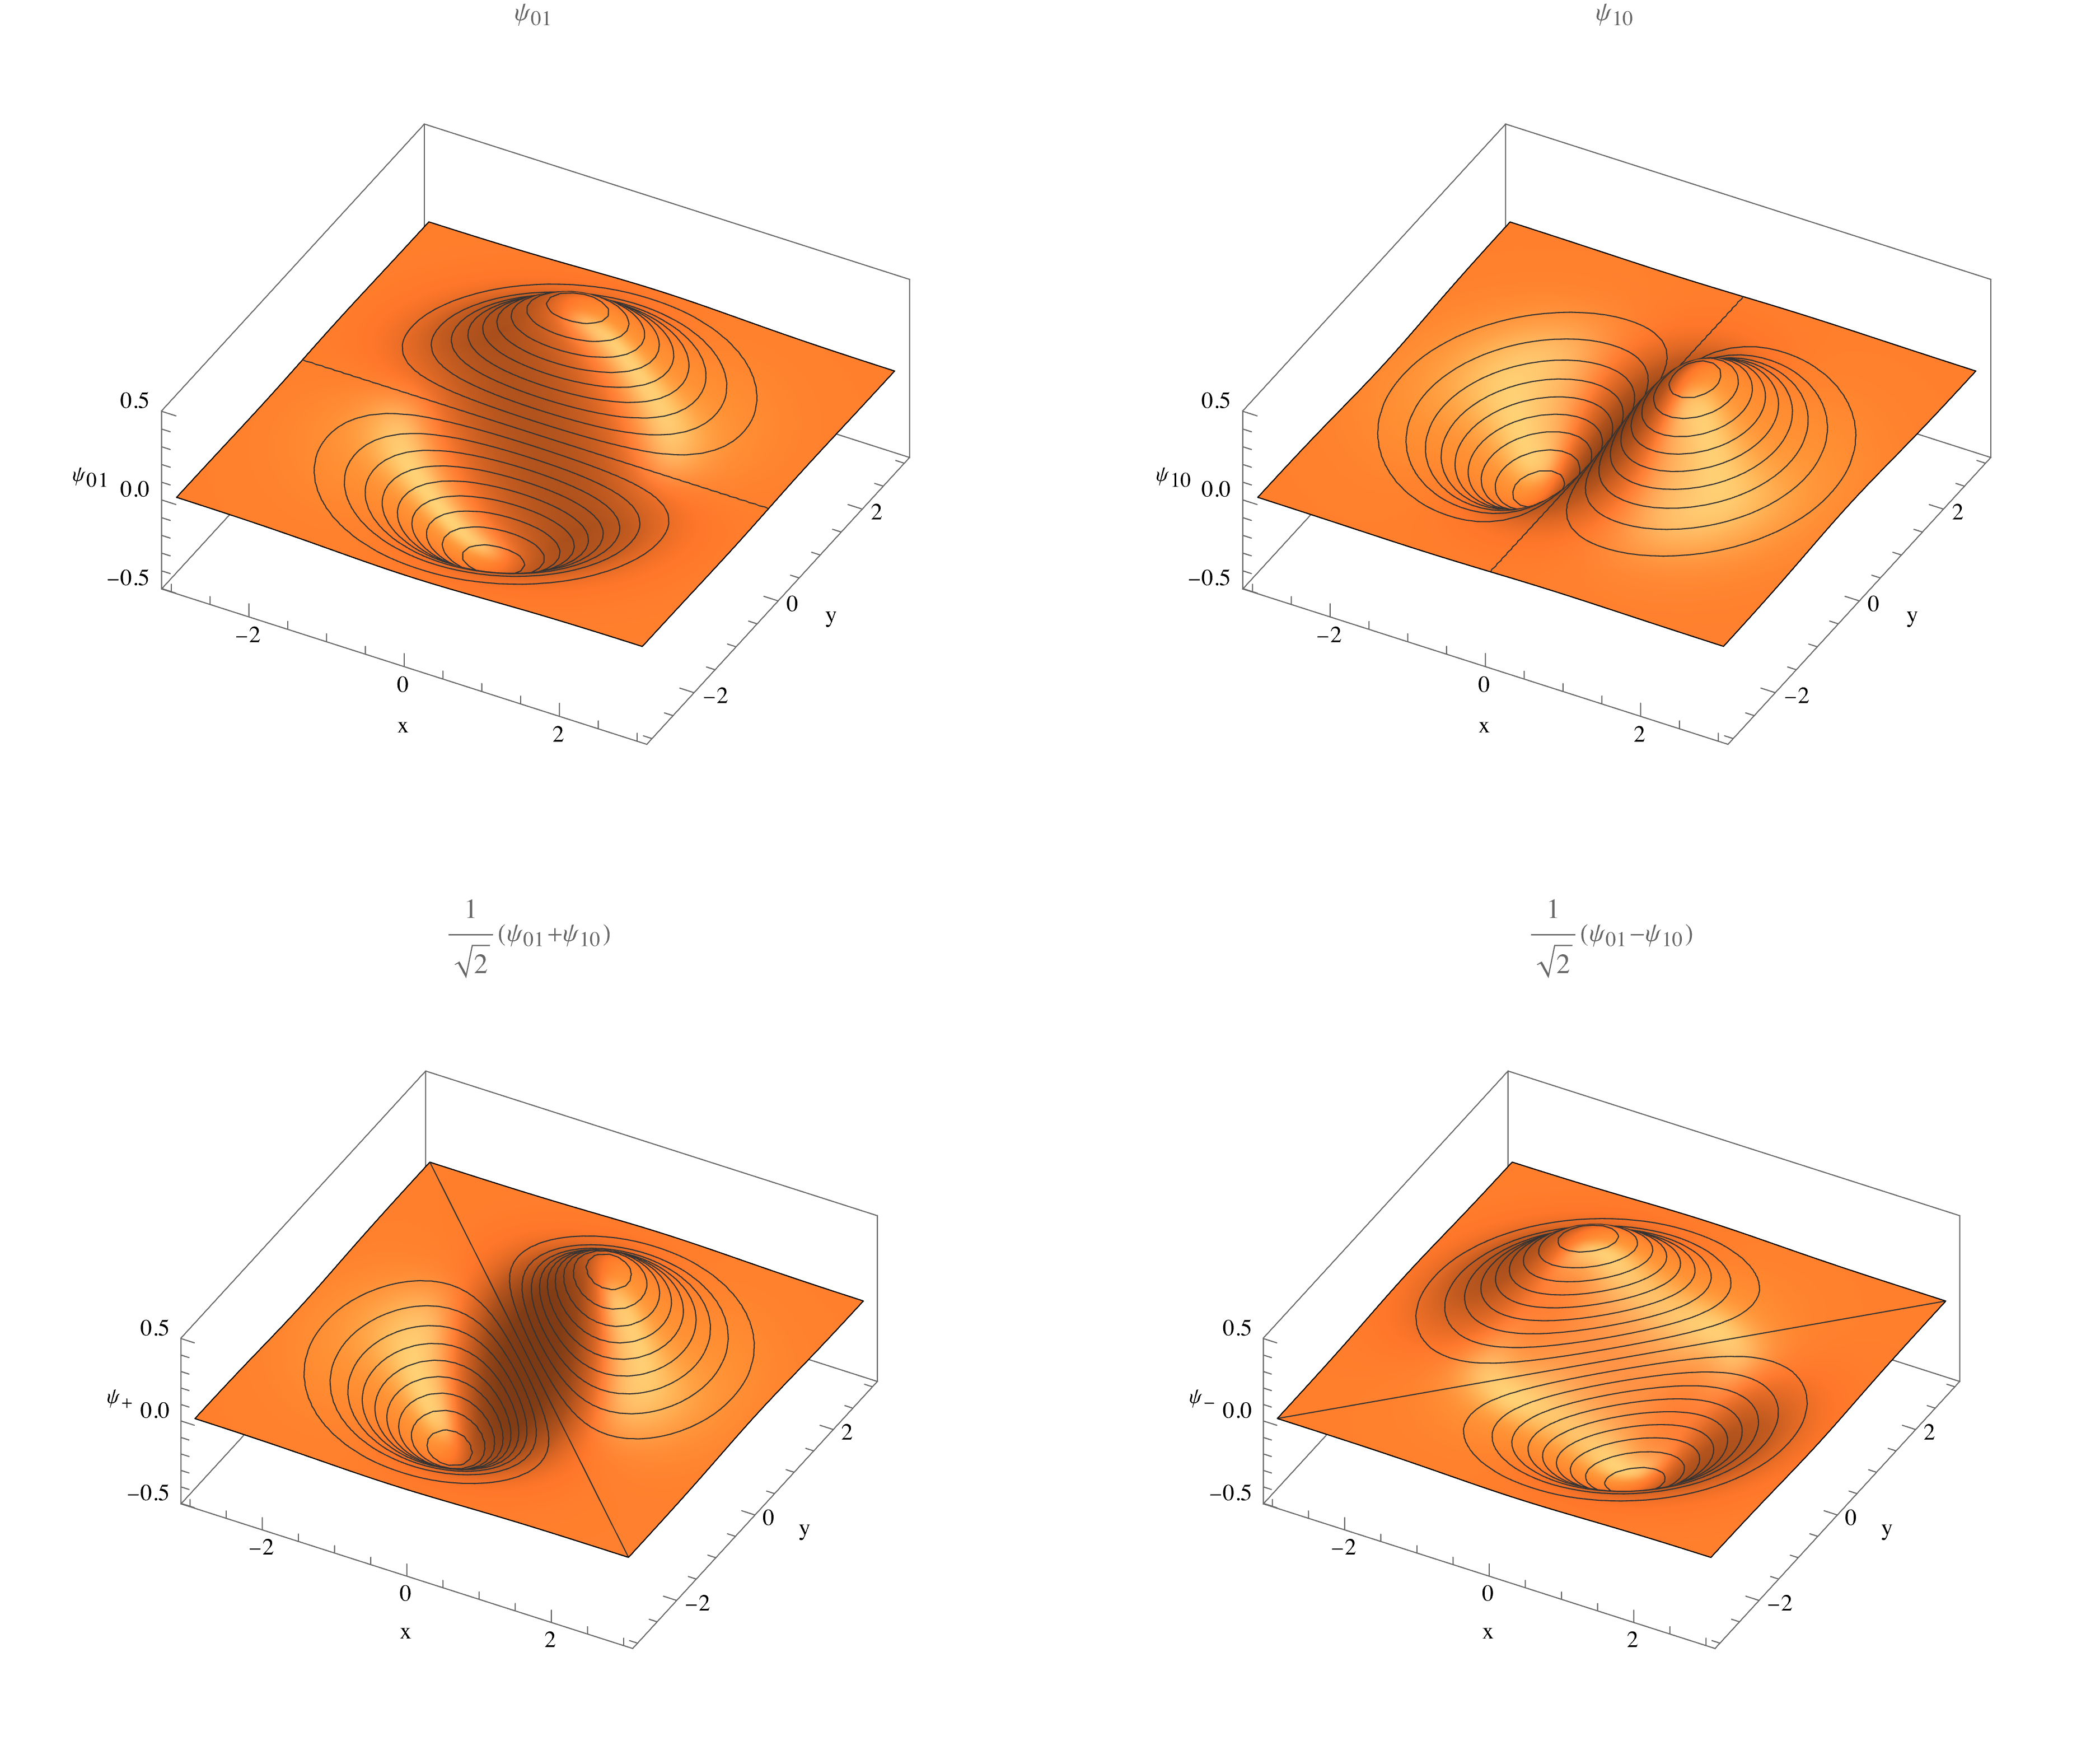
\includegraphics[width=\linewidth]{fig/grid.png}
\caption{Number states $\ket{\psi_{01}},\ket{\psi_{10}}$ and `good' states $\ket{\psi_{+}},\ket{\psi_{-}}$ in the position representation.
\label{visualizingGoodStates}
}
\end{figure}
From these results, the second-order corrections energies are,
\begin{align}
	E_- 
	&=
	2 \hbar \omega
	-
	\frac{\hbar \lambda}{2 m \omega}
	-
	\frac{\hbar \lambda^2}{4 m^2 \omega^3}
	+
	O((\tfrac{\lambda}{m \omega^2})^3),
	\\
	E_+
	&=
	2 \hbar \omega
	+
	\frac{\hbar \lambda}{2 m \omega}
	-
	\frac{\hbar \lambda^2}{4 m^2 \omega^3}
	+
	O((\tfrac{\lambda}{m \omega^2})^3).
\end{align}
To find the first-order corrected states, we must normalize the states:
\begin{align}
	\ket{\psi_-'}
	&=
	\frac{1}{\sqrt{
		1+
		\frac{1}{2}
		\left(
			\frac{\lambda}{2m \omega^2}
		\right)^2
	}}
	\left(
	\frac{1}{\sqrt{2}}
	(
		\ket{\psi_{01}}
		-
		\ket{\psi_{10}}
	)
	+
	\frac{\lambda}{4m \omega^2}
	(
		\ket{\psi_{21}}
		-
		\ket{\psi_{12}}
	)
	+
	O((\tfrac{\lambda}{m \omega^2})^2)
	\right),
	\\
	\ket{\psi_-'}
	&=
	\frac{1}{\sqrt{
		1+
		\frac{1}{2}
		\left(
			\frac{\lambda}{2m \omega^2}
		\right)^2
	}}
	\left(
	\frac{1}{\sqrt{2}}
	(
		\ket{\psi_{01}}
		-
		\ket{\psi_{10}}
	)
	-
	\frac{\lambda}{4m \omega^2}
	(
		\ket{\psi_{21}}
		+
		\ket{\psi_{12}}
	)
	+
	O((\tfrac{\lambda}{m \omega^2})^2)
	\right)
\end{align}


\paragraph{Exact solution}

By changing coordinates, we can solve this problem exactly!
If we use rotated coordinates $u,v$ so that,
\begin{align}
	u &= \frac{1}{\sqrt{2}}(x + y),
	\qquad
	v = \frac{1}{\sqrt{2}}(x - y),
	\\
	x &= \frac{1}{\sqrt{2}}(u + v),
	\qquad
	y = \frac{1}{\sqrt{2}}(u - v),
\end{align}
the perturbed Hamiltonian becomes,
\begin{align}
	\hat H
	=
	\hat H_0
	+
	\hat H'
	&=\nonumber
	\frac{1}{2m} ( \hat p_u^2 + \hat p_v^2)
	+
	\frac{1}{4} m \omega^2
	\left(
		(u+v)^2
		+
		(u-v)^2
	\right)
		+
	\lambda
	(u+v)
	(u-v)
	\\
	&=
	\frac{1}{2m} ( \hat p_u^2 + \hat p_v^2)
	+
	\frac{1}{2} m \omega^2
	\left[
		\left(
			1 + \frac{\lambda}{m \omega^2}
		\right)
		u^2
		+
		\left(
			1 - \frac{\lambda}{m \omega^2}
		\right)
		v^2
	\right],
\end{align}
so we have now have a non-isotropic two-dimensional harmonic oscillator.
In the $u$-direction, $\omega_u = \omega \sqrt{1+ \lambda/(m \omega^2)}$, and in the $v$-direction $\omega_v = \omega \sqrt{1- \lambda/(m \omega^2)}$.
This means that the exact energies and their power series expansion are,
\begin{align}
	E_{n_u,n_v}
	&=
	\hbar \omega
	\left[
		\sqrt{1+\frac{\lambda}{m \omega^2}}
		\left(
		n_u + \frac{1}{2}	
		\right)
		+
		\sqrt{1-\frac{\lambda}{m \omega^2}}
		\left(
		n_v + \frac{1}{2}	
		\right)
	\right]
	\\
	&=
	\hbar \omega 
	\left(
		1+ n_u + n_v
	\right)
	+
	\lambda
	\frac{\hbar (n_u - n_v)}{2 m \omega}
	-
	\lambda^2
	\frac{\hbar (1+ n_u + n_v)}{8 m^2 \omega^3}
	+ 
	O(\lambda^3)
	,
\end{align}
where $(n_u,n_v) = (0,0),(1,0),(0,1),(1,1),\dots$ are the quantum numbers.
If we substitute quantum numbers $(n_u,n_v) = (0,1)$ or  $(n_u,n_v) = (1,0)$ into the power series expansion, we see that we successfully recover our perturbative approximations!







\end{document}






